\documentclass[letterpaper,11pt]{article}

\usepackage{listings}
\usepackage{color}

\definecolor{dkgreen}{rgb}{0,0.6,0}
\definecolor{gray}{rgb}{0.5,0.5,0.5}
\definecolor{mauve}{rgb}{0.58,0,0.82}

\lstset{frame=tb,
  language=Python,
  aboveskip=3mm,
  belowskip=3mm,
  showstringspaces=false,
  columns=flexible,
  basicstyle={\small\ttfamily},
  numbers=none,
  numberstyle=\tiny\color{gray},
  keywordstyle=\color{blue},
  commentstyle=\color{dkgreen},
  stringstyle=\color{mauve},
  breaklines=true,
  breakatwhitespace=true,
  tabsize=3
}

\usepackage{setspace}
\usepackage{graphicx}
\usepackage{bm}    %for textbf
\usepackage{amsmath}
\usepackage{amsfonts}   %for mathbb
\allowdisplaybreaks[4]  %from {amsmath}
\newcommand{\independent}{\rotatebox[origin=c]{90}{$\models$}}  %from {graphicx}
\usepackage{geometry}
\geometry{letterpaper, scale=0.8}  %from {geometry}
\author{Yuan Yin}
\title{MATH 623 Homework 3}
\begin{document}\large
\maketitle
\begin{spacing}{1.2}  %from {setspace}
\section*{Problem 1}
\subsection*{4. \& 5.}
The main code:
\begin{lstlisting}
r = 0.02; sigma = 0.2; K = 1; T = 1; N = 100;
a = log(K) - 3 * sigma * T^0.5 - (r - sigma^2 / 2) * T;
b = log(K) + 3 * sigma * T^0.5 + abs(r - sigma^2 / 2) * T;
M = 556; dt = T / M; dx = (b - a) / N; u = zeros(M + 1, N + 1);
alpha0 = 1 - sigma^2 * dt / dx^2;
alpha1 = sigma^2 * dt / (2 * dx^2) + (r - sigma^2 / 2) * dt / dx / 2;
alpha2 = sigma^2 * dt / (2 * dx^2) - (r - sigma^2 / 2) * dt / dx / 2;
for i = 1 : (N + 1)
    u(1, i) = max(0, K - exp(a + (i - 1) * dx));
end
for i = 1 : (M + 1)
    u(i, 1) = K * exp(- r * (T - dt * (i - 1))) - exp(a);
    u(i, N + 1) = 0;
end
for i = 2 : (M + 1)
    for j = 2 : N
        u(i, j) = max(K - exp(a + dx * (j - 1)), (alpha0 - r * dt) * u(i - 1, j) + alpha1 * u(i - 1, j + 1) + alpha2 * u(i - 1, j - 1));
    end
end
x = a: dx : b; s = exp(x);
figure(1)
plot(s, u(M + 1, :))
Ex = [];
for i = (M + 1) : -1 : 1
    p = [];
    for j = 1 : (N + 1)
        if (u(i, j) > (K - exp(a + dx * (j - 1))))
            p = [p, exp(a + dx * (j - 1))];
        end
    end
    Ex = [Ex, min(p)];
end
t = 0 : dt : T;
figure(2)
plot(t, Ex)
\end{lstlisting}

the plot of $V(S,0)$ is as below:

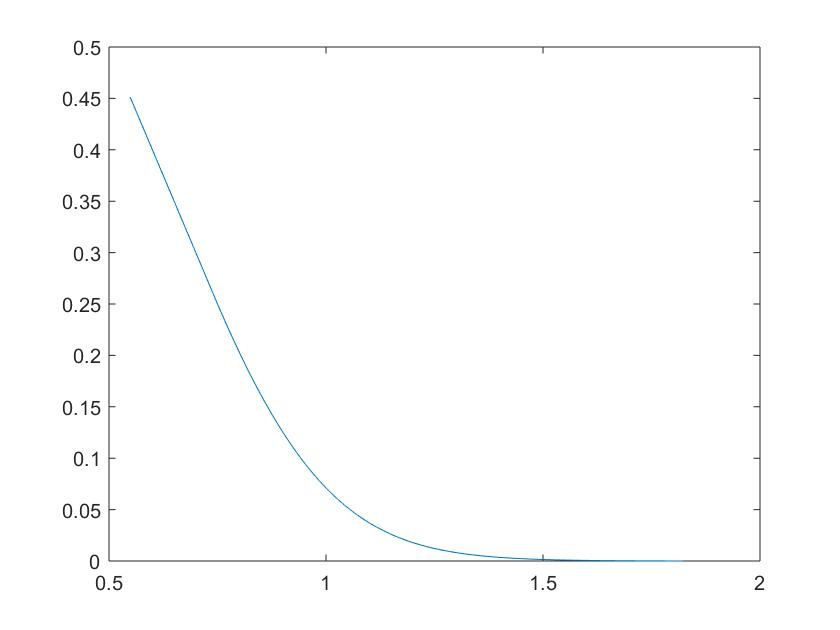
\includegraphics[width=4.95in,height=3.95in]{problem1_4.jpg}

the plot of $(Ex_m)_{0 \leq m \leq M}$ is as below:

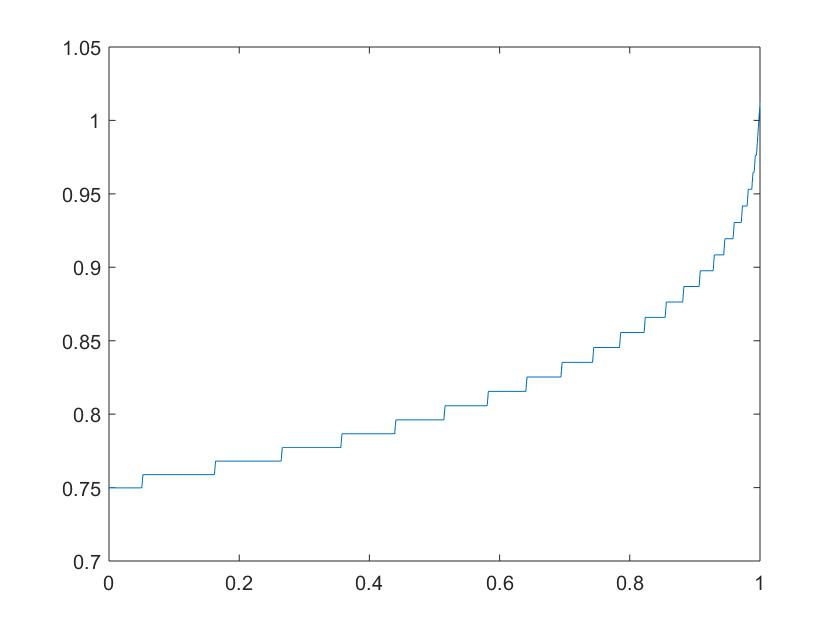
\includegraphics[width=4.95in,height=3.95in]{problem1_5.jpg}

\section*{Problem 2}
\subsection*{3. \& 4.}
The main code:
\begin{lstlisting}
r = 0.02; sigma = 0.2; K = 1; T = 1; L = 0.5; N = 100; M = 556;
a = log(L); b = log(K) + 3 * sigma * T^0.5 + abs(r - sigma^2 / 2) * T;
dt = T / M; dx = (b - a) / N;
alpha0 = 1 - sigma^2 * dt / dx^2;
alpha1 = sigma^2 * dt / (2 * dx^2) + (r - sigma^2 / 2) * dt / dx / 2;
alpha2 = sigma^2 * dt / (2 * dx^2) - (r - sigma^2 / 2) * dt / dx / 2;
for i = 1 : (N + 1)
    u(1, i) = max(0, exp(a + (i - 1) * dx) - K);
end
for i = 1 : (M + 1)
    u(i, N + 1) = exp(b) - K * exp(- r * (T - dt * (i - 1)));
    u(i, 1) = 0;
end
for i = 2 : (M + 1)
    for j = 2 : N
        u(i, j) = (alpha0 - r * dt) * u(i - 1, j) + alpha1 * u(i - 1, j + 1) + alpha2 * u(i - 1, j - 1);
    end
end
x = a: dx : b; s = exp(x);
figure(1)
plot(s, u(M + 1, :))

[call_1,put_1] = blsprice(1, K, r, T, sigma);
[call_L2, put_L2] = blsprice(L^2, K, r, T, sigma);
real_p = call_1 - L^(2 * r / sigma^2 - 1) * call_L2;
m = 1056 : -1 : 556;
delta_t = []; error = [];
for i = 1 : length(m)
    delta_t = [delta_t, T / m(i)];
    est_p = est_of_p(T / m(i));
    error = [error, abs(real_p - est_p)];
end
figure(2)
plot(delta_t, error)
\end{lstlisting}

and the function code:
\begin{lstlisting}
function y = est_of_p(x)
r = 0.02; sigma = 0.2; K = 1; T = 1; L = 0.5; N = 100; M = fix(T / x);
a = log(L); b = log(K) + 3 * sigma * T^0.5 + abs(r - sigma^2 / 2) * T;
dt = T / M; dx = (b - a) / N;
alpha0 = 1 - sigma^2 * dt / dx^2;
alpha1 = sigma^2 * dt / (2 * dx^2) + (r - sigma^2 / 2) * dt / dx / 2;
alpha2 = sigma^2 * dt / (2 * dx^2) - (r - sigma^2 / 2) * dt / dx / 2;
for i = 1 : (N + 1)
    u(1, i) = max(0, exp(a + (i - 1) * dx) - K);
end
for i = 1 : (M + 1)
    u(i, N + 1) = exp(b) - K * exp(- r * (T - dt * (i - 1)));
    u(i, 1) = 0;
end
for i = 2 : (M + 1)
    for j = 2 : N
        u(i, j) = (alpha0 - r * dt) * u(i - 1, j) + alpha1 * u(i - 1, j + 1) + alpha2 * u(i - 1, j - 1);
    end
end
for i = 1 : (N + 1)
    if ((a + dx * (i - 1) < 0) & (a + dx * i >= 0))
        q = i;
    end
end
y = u(M + 1, q + 1);
end
\end{lstlisting}

the plot of $V(S,0)$ is as below:

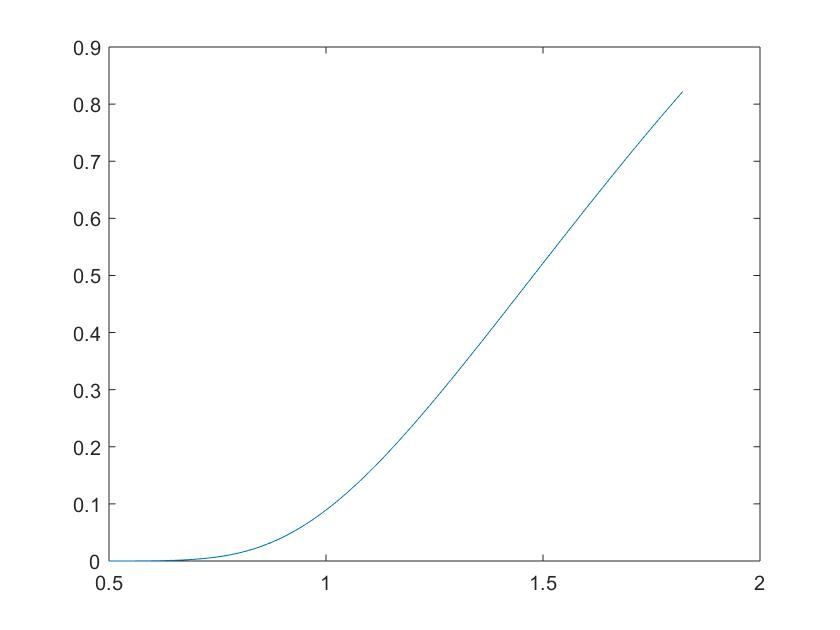
\includegraphics[width=4.95in,height=3.95in]{problem2_3.jpg}

the plot of error is as below:

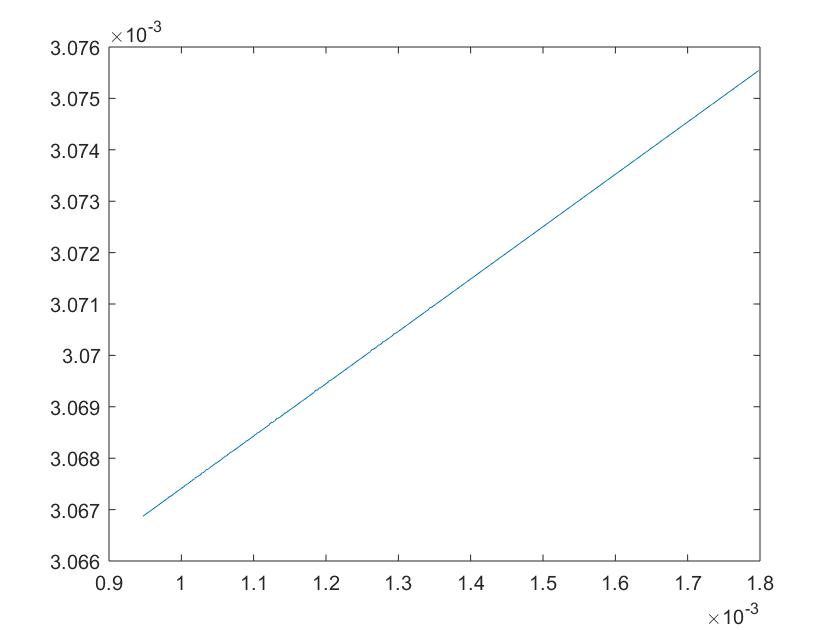
\includegraphics[width=4.95in,height=3.95in]{problem2_4.jpg}
\end{spacing}
\end{document}